\chapter{Introduction}

\section{Motivation}
From proposal: \\
The	 goal	 is	 to	 visualize	 a	 hierarchical	 network	 with	 n	 Layers.	 Each	 Node	 in	 a	 graph	 can	
represent	a	graph	itself.	There	are	multiple	examples	where	this	has	been	visualised	in	2D,	
however	we	believe	that	with	an	additional	dimension	and	when	3D	graphs	are	analysed	in	
VR	we	can	get	even	more	insight	and	a	better	overview	of	the	data.	

\textbf{Starting idea: 2D Multilayer see figure, why not make use of all 3 axes in VR, instead of flat layers use 3D objects like cubes/spheres to bundle one layer} (Email 14.08.2020 https://arxiv.org/pdf/1902.06815.pdf)
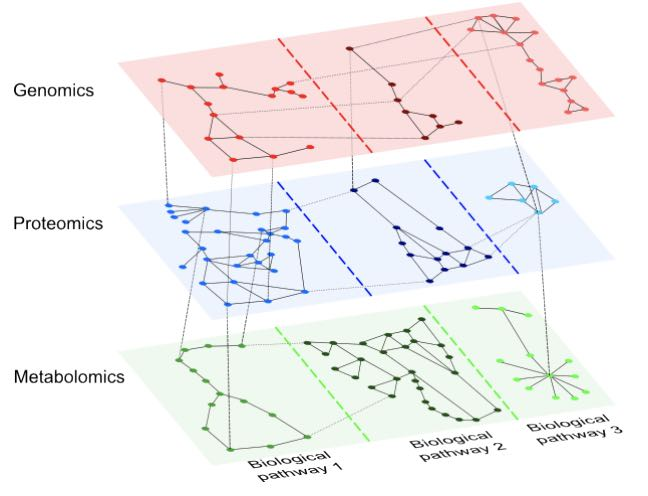
\includegraphics[width=0.5\textwidth]{chapters/graphics/2dmultilayerVis.jpg}

Ideas:
\begin{itemize}
    \item Example applications with hierarchical network data
    \item current 2D visualizations of hierarchical networks
    \item power of VR visualizations and board availability
\end{itemize}

\section{Aim of the Work}

Ideas:
\begin{itemize}
    \item provide a prototype application
    \item benefits of webbased implementation 
    \item experiment with different concepts/approaches
    \item experiment with different interactions
    \item ...
\end{itemize}

\begin{quotation}
    However, there is considerable value in research that
    solves a well-motivated problem using a combination
    of preexisting solutions 
\end{quotation}
Sadana\\
Redefining a Contribution for Immersive Visualization Research\\

\section{Approach}

I want to give a short summary of chapter 4 proposed solution here. 

Ideas:
\begin{itemize}
    \item short description of planned final solution (web based, htc vive compatible, rendering multi hierarchical dataset, screenshot of solution)  
    \item short overview of used technologies and frameworks why? what it simplifies, ... 
    \item Customized Forces
    \item rendering, nodes inside parent, comparison to a default 2D Circle Packing plot https://observablehq.com/@d3/zoomable-circle-packing 
    \item available interactions
\end{itemize}